\documentclass[10pt]{beamer}

\usetheme[progressbar=frametitle]{metropolis}
\usepackage{appendixnumberbeamer}
\usepackage[utf8]{inputenc}

\usepackage{multicol}
\usepackage{booktabs}
\usepackage[scale=2]{ccicons}
\usepackage{color}

\usepackage{pgfplots}
\usepgfplotslibrary{dateplot}

\usepackage{xspace}
\newcommand{\themename}{\textbf{\textsc{metropolis}}\xspace}

\title{IA para el Desarrollo de Videojuegos}
\subtitle{Proyecto final: \\Real Time Wargame.}
% \date{\today}
\date{}
\author{Autores: \\Antonio López Martínez-Carrasco \\José María Sánchez Salas}
\institute{Profesores: \\Francisco Javier Marín-Blazquez Gómez \\Luis Daniel Hernández Molinero}
% \titlegraphic{\hfill\includegraphics[height=1.5cm]{logo.pdf}}

\begin{document}

\maketitle

\section{Introducción}

\begin{frame}{Introducción}
\begin{itemize}[<+- | alert@+>]
 \item Software y Hardware utilizado.
 \begin{itemize}[<+- | alert@+>]
  \item Librería LibGDX (implementada en Java).
  \item IDE Eclipse.
  \item Ningún hardware específico.
 \end{itemize}
\end{itemize}
\end{frame}

\section{Modelo}

\begin{frame}{Modelo}
\begin{itemize}[<+- | alert@+>]
	\item Clase abstracta WorldObject.
	\begin{itemize}
	 \item Hereda de Sprite (librería LibGDX).
	\end{itemize}
	\item Obstacle.
	\begin{itemize}
	 \item Hereda de WorldObject.
	 \item Obstáculos \textbf{estáticos}.
	\end{itemize}

	\item Character.
	\begin{itemize}
	 \item Hereda de WorldObject.
	 \item Personajes del mundo.
	\end{itemize}

	\item Formation:
	\begin{itemize}[<+- | alert@+>]
		\item Hereda de Character.
  		\item CircularFormation.
  		\item LineFormation.
  		\item StarFormation \href{videos/TestStarFormation.mp4}{\color{blue}\underline{Video}} 
 	\end{itemize}
 \end{itemize}
\end{frame}


\begin{frame}{Modelo -- Formaciones}
\begin{itemize}[<+- | alert@+>]
	\item Patrón de diseño Composite.
	\item Patrón de diseño Método Plantilla.
	\item Cierta funcionalidad se delega a las formaciones concretas:
	\begin{itemize}
	 \item Calcular la posición de los integrantes.
	 \item Calcular el Steering a aplicar (árbitro y lista de comportamientos ``a pelo'').
	\end{itemize}

	\item La lista de comportamientos de los integrantes no se tiene en cuenta.
	\item El movimientos de los integrantes a sus respectivas posiciones se hace con una lista de comportamientos ``a pelo'' (utilizando un árbitro por prioridad, se explica más adelante).
 \end{itemize}
\end{frame}

\begin{frame}{Modelo -- Formaciones}
\begin{figure}[!th]
 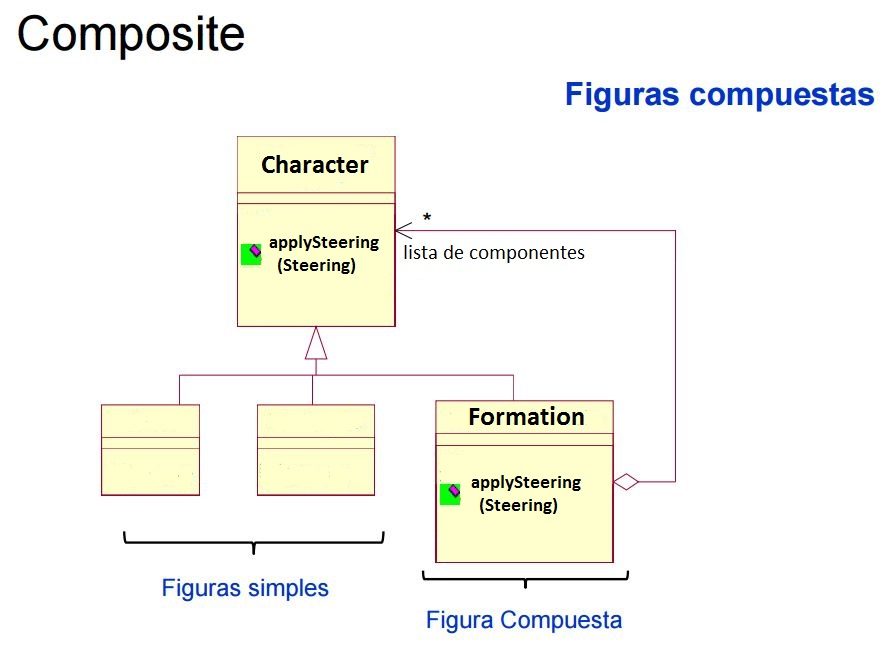
\includegraphics[scale=0.38]{images/composite}
\end{figure}
\end{frame}

\begin{frame}{Modelo -- Ejemplo formación compleja}
\begin{itemize}
 \item \href{videos/TestComplexFormation.mp4}{\color{blue}\underline{Video}} 
\end{itemize}
\end{frame}



\section{Steerings}
\begin{frame}{Steerings}
\begin{itemize}[<+- | alert@+>]
	\item Interfaz Steering.
	\begin{itemize}[<+- | alert@+>]
  		\item Para tratar a todos los tipos de Steerings de manera homogénea.
 	\end{itemize}
 	\item Steerings no acelerados.
 	\begin{itemize}[<+- | alert@+>]
  		\item Velocidad lineal y velocidad angular.
 	\end{itemize}
 	\item Steerings acelerados.
 	\begin{itemize}[<+- | alert@+>]
  		\item Aceleración lineal y aceleración angular.
 	\end{itemize}
\end{itemize}
\end{frame}

\section{Comportamientos}
\begin{frame}{Comportamientos}
\begin{itemize}[<+- | alert@+>]
	\item Interfaz Behaviour.
	\begin{itemize}[<+- | alert@+>]
  		\item Para tratar a todos los tipos de comportamientos de manera homogénea.
  		\item Método \texttt{getSteering()}.
 	\end{itemize}
 	\item Behaviours no acelerados.
 	\begin{itemize}[<+- | alert@+>]
  		\item Seek \item Flee \item Arrive \item Wander 
 	\end{itemize}
 	\item Behaviours acelerados.
 	\begin{itemize}[<+- | alert@+>]
  		\item Align \item Anti-Align \item Arrive con un radio \href{videos/TestArrive\_Accelerated\_WithOneRadious.mp4}{\color{blue}\underline{Video}}
  		\item Arrive \item Flee \item Seek \item Velocity Matching
 	\end{itemize}
\end{itemize}
\end{frame}

\begin{frame}{Comportamientos}
\begin{itemize}[<+- | alert@+>]
	\item Behaviours delegados.
 	\begin{itemize}[<+- | alert@+>]
  		\item CollisionAvoidance \item Evade \item Face \item Looking Where You Going \item PathFollowing con Arrive 
  		\item PathFollowing con Seek \href{videos/TestPathFollowingWithoutPathOffset.mp4}{\color{blue}\underline{Video}}
  		\item Persue \href{videos/TestPersue.mp4}{\color{blue}\underline{Video}}
  		\item WallAvoidance \item Wander 
 	\end{itemize}
 	\item Behaviours en grupo.
 	\begin{itemize}[<+- | alert@+>]
  		\item Cohesion \href{videos/TestCohesion.mp4}{\color{blue}\underline{Video}}
  		\item Separation \href{videos/TestSeparation.mp4}{\color{blue}\underline{Video}}
 	\end{itemize}
\end{itemize}
\end{frame}


\section{Árbitros}
\begin{frame}{Árbitros}
\begin{itemize}[<+- | alert@+>]
	\item Interfaz Arbitrator.
	\begin{itemize}[<+- | alert@+>]
  		\item Para tratar a todos los tipos de árbitros de manera homogénea.
  		\item Método \texttt{getSteering(behaviours)}.
 	\end{itemize}
	\item Lista de comportamientos de los personajes.
	\begin{itemize}[<+- | alert@+>]
  		\item Mapa con clave Float y valor Behaviour.
  		\item Ordenados de mayor a menor $\rightarrow$ Más importante primero.
 	\end{itemize}
	
	\item Árbitro por prioridad.
	\begin{itemize}[<+- | alert@+>]
  		\item Para comportamientos acelerados y no acelerados.
  		\item Ejecuta los comportamientos siguiendo su orden.
  		\item Devuelve el Steering de un comportamiento si supera cierto valor \texttt{epsilon}.
  		\item Si llega al final, devuelve el último de la lista.
 	\end{itemize}
	\item Árbitro por mezcla. Comportamientos acelerados.
	\item Árbitro por mezcla. Comportamientos no acelerados.
\end{itemize}
\end{frame}

\section{Interacción parte Reactiva}
\begin{frame}{Interacción parte Reactiva}
\begin{itemize}[<+- | alert@+>]
	\item Método \texttt{applyBehaviour()}.
	\begin{itemize}[<+- | alert@+>]
	 \item Si el personaje no pertenece a una formación, se invoca a su árbitro.
	 \item Se llama al método \texttt{applySteering(steering)} con el Steering devuelto.
	\end{itemize}

	\item Método \texttt{applySteering(steering)}.
	\begin{itemize}[<+- | alert@+>]
	 \item Si el personaje no pertenece a una formación, se invoca al método \texttt{update(steering, time)}.
	\end{itemize}

	\item Método \texttt{update(steering, time)}.
	\begin{itemize}[<+- | alert@+>]
	 \item Se actualizan los parámetros del personaje en función del Steering.
	\end{itemize}

\end{itemize}
\end{frame}

\section{PathFinding}
\begin{frame}{PathFinding}
\begin{itemize}[<+- | alert@+>]
 
  \item PathFinding con algoritmo LRTA* y espacio de búsqueda minimal.
  \item Distancias Ecluidea, Chebyshev y Manhattan.
  
  \item PathFinding Continuo.
  \begin{itemize}[<+- | alert@+>]
   \item Devuelve la \textbf{lista completa} de puntos desde el origen al destino.
   \item Solo es necesario llamarlo una vez.
  \end{itemize}

  \item PathFinding Punto-A-Punto.
	\begin{itemize}[<+- | alert@+>]
  		\item Va devolviendo \textbf{punto por punto}.
  		\item Se debe llamar continuamente para obtener al punto al que ir.
 	\end{itemize}
\end{itemize}
\end{frame}


\section{Modificaciones del modelo para la parte Táctica}
\begin{frame}{Clase Character}
\begin{itemize}[<+- | alert@+>]
	\item Nuevos atributos.
	\begin{itemize}[<+- | alert@+>]
  		\item Rol táctico.
  		\item Vida (máxima y actual).
  		\item Equipo.
 	\end{itemize}
	\item Nuevos métodos.
	\begin{itemize}[<+- | alert@+>]
  		\item \texttt{initializeTacticalRole(role)}.
  		\item \texttt{updateTacticalRole()}.
  		\item \texttt{getVelocityFactorOfThisCharacter()} (se explica más adelante).
 	\end{itemize}
\end{itemize}
\end{frame}

\begin{frame}{Enumerado Team}
\begin{itemize}[<+- | alert@+>]
	\item Equipos del juego.
	\begin{itemize}[<+- | alert@+>]
  		\item \texttt{FJAVIER}.
  		\item \texttt{LDANIEL}.
  		\item \texttt{NEUTRAL}.
 	\end{itemize}
	\item Método \texttt{getEnemyTeam()}.
\end{itemize}
\end{frame}

\section{Roles Tácticos}
\begin{frame}{Roles Tácticos}
\begin{itemize}[<+- | alert@+>]
	\item Interfaz TacticalRole.
	\item Clases abstractas Archer y Soldier.
	\item Roles defensivos.
	\begin{itemize}[<+- | alert@+>]
  		\item Soldado y arquero.
 	\end{itemize}
 	\item Roles ofensivos.
	\begin{itemize}[<+- | alert@+>]
  		\item Soldado y arquero.
 	\end{itemize}
\end{itemize}
\end{frame}

\begin{frame}{Interfaz TacticalRole}
\begin{itemize}[<+- | alert@+>]
	\item Métodos.
	\begin{itemize}[<+- | alert@+>]
  		\item \texttt{getVelocityFactor(ground)} (es usado en la clase Character).
  		\item \texttt{getTacticalCost(ground)}.
  		\item \texttt{getMaxDistanceOfAttack()}.
  		\item \texttt{getDamageToDone()}.
  		\item \texttt{getMaxSpeed()}.
  		\item \texttt{initialize(character)}.
  		\item \texttt{update(character)}.
  		\item Estos métodos son implementados en las clases abstractas Archer y Soldier.
 	\end{itemize}
 	\item Atributo \texttt{health\_cure}.
 	\begin{itemize}[<+- | alert@+>]
  		\item Todos se curan al mismo ritmo, independientemente de su rol.
 	\end{itemize}
\end{itemize}
\end{frame}

\begin{frame}{Roles Defensivos}
\begin{itemize}[<+- | alert@+>]
	\item Soldado.
\end{itemize}
\begin{figure}[!th]
	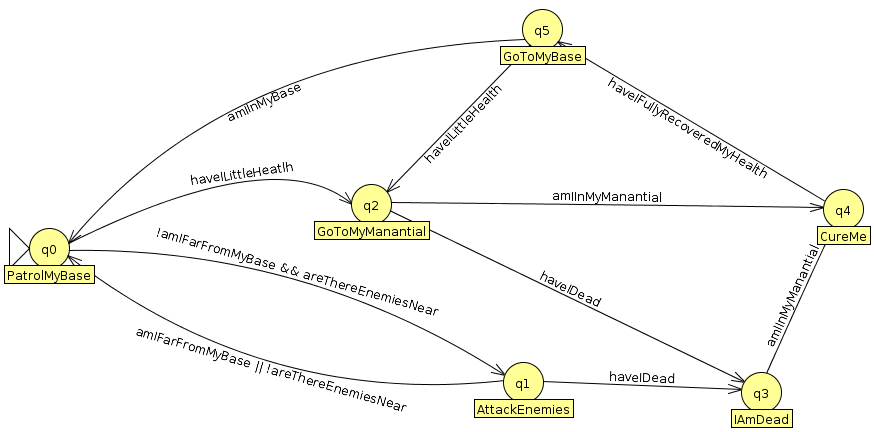
\includegraphics[scale=0.38]{images/defensive-soldier}
\end{figure}
\end{frame}

\begin{frame}{Roles Defensivos}
\begin{itemize}[<+- | alert@+>]
	\item Arquero.
\end{itemize}
\begin{figure}[!th]
	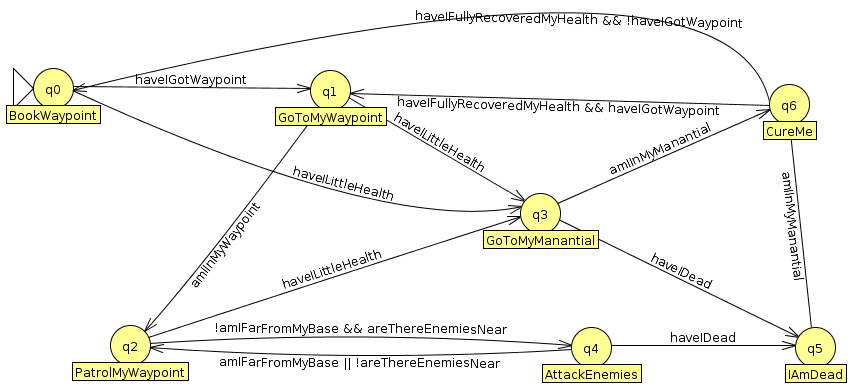
\includegraphics[scale=0.38]{images/defensive-archer}
\end{figure}
\end{frame}

\begin{frame}{Roles Ofensivos}
\begin{itemize}[<+- | alert@+>]
	\item Soldado y arquero.
\end{itemize}
\begin{figure}[!th]
	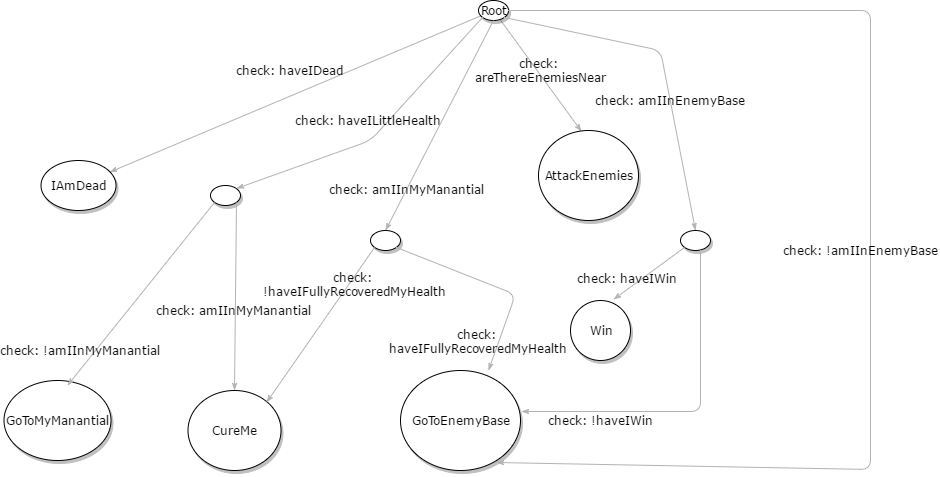
\includegraphics[scale=0.35]{images/arbolDecisionOfensivo}
\end{figure}
\end{frame}


\section{Otros comportamientos}
\begin{frame}{Otros comportamientos}
\begin{itemize}[<+- | alert@+>]
	\item Ataque.
	\item Cura.
	\item Se han implementado como Behaviours para tratarlos de manera homogénea.
	\item Ataque y Cura en las formaciones.
	\begin{itemize}[<+- | alert@+>]
	 \item El ancla es el que da las órdenes de ataque y cura a los integrantes.
	\end{itemize}

\end{itemize}
\end{frame}


\section{Acciones y comprobaciones}
\begin{frame}{Acciones y comprobaciones}
\begin{itemize}[<+- | alert@+>]
	\item Actions.
	\item Checks.
	\item Útiles para la abstracción de la parte reactiva.
	\item Sirven de puente entre la parte reactiva y la parte táctica.
\end{itemize}
\end{frame}


\section{Waypoints}
\begin{frame}{Waypoints}
\begin{itemize}[<+- | alert@+>]
	\item Waypoints de las bases.
	\item Waypoints de los puentes.
	\begin{itemize}[<+- | alert@+>]
		\item Cada equipo tiene 6 waypoints.
		\item En cada lado de los puentes, hay 2 waypoints.
		\item Sistema de reserva y liberación de waypoints.
	\end{itemize}
\end{itemize}
\end{frame}


\section{Puntos de Moral}
\begin{frame}{Puntos de Moral}
\begin{itemize}[<+- | alert@+>]
	\item Cada base tiene una puntuación de moral.
	\item La moral de una base sube cuando hay personajes de un equipo en su base y no hay personajes del equipo contrario.
	\item La moral de una base baja cuando la base no está protegida y hay personajes del equipo contrario.
	\item El equipo ganador es el que consigue reducir los puntos de moral de la base contraria a 0.
\end{itemize}
\end{frame}

\section{Mapas de Influencia}
\begin{frame}{Mapas de Influencia}
\begin{itemize}[<+- | alert@+>]
	\item El mapa de influencia refleja la presencia/poder de un equipo en una zona.
	\item Cada equipo tiene su propio mapa/matriz de influencia.
	\item El equipo con mayor influencia en una casilla, domina dicha casilla.
	\item La influencia se va reduciendo con la distancia.
	\item Para el cálculo de la influencia se ha utilizado la distancia de Chebyshev (con algunas modificaciones).
	\item Al dibujar el mapa se tienen en cuenta ambas matrices de influencia.
\end{itemize}
\end{frame}

\begin{frame}{Mapas de Influencia}
\begin{figure}[!th]
	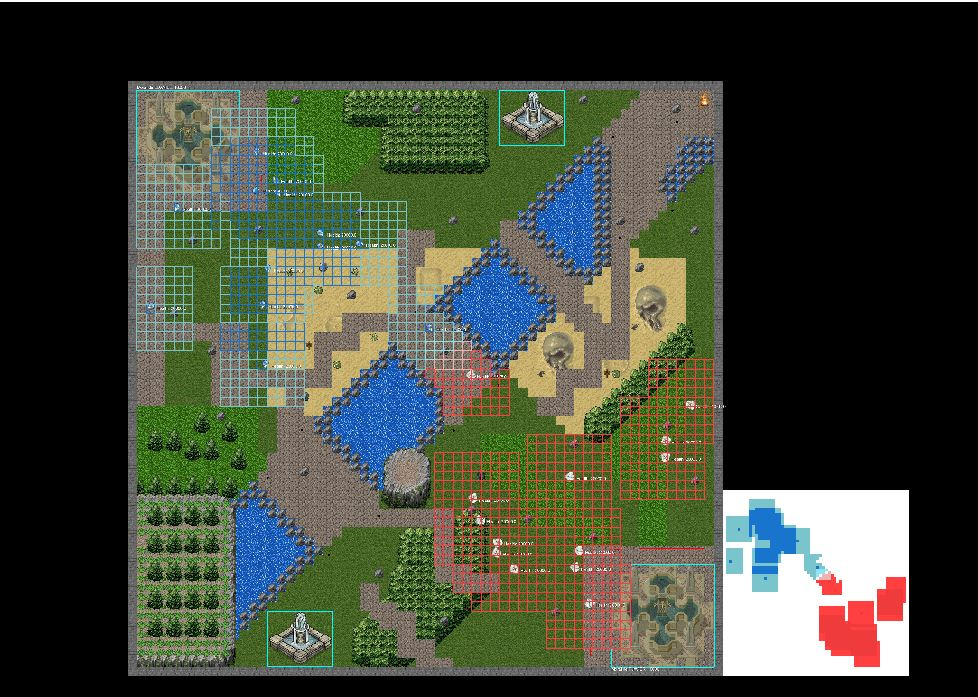
\includegraphics[scale=0.4]{images/influencia}
\end{figure}
\end{frame}

\section{PathFinding Táctico}
\begin{frame}{PathFinding Táctico}
\begin{itemize}[<+- | alert@+>]
	\item Hace uso de los mapas de influencia.
	\item También puede hacer uso de la información táctica (\texttt{getTactialCost(ground)}) de cada rol.
	\item Flag para que se pueda ir activando y desactivando sobre la marcha.
	\item \href{videos/TestTacticalPathfinding\_(SIN\_COLISIONES).mp4}{\color{blue}\underline{Video}} (sin colisiones)
\end{itemize}
\end{frame}


\section{Flocking}
\begin{frame}{Flocking}
\begin{itemize}[<+- | alert@+>]
	\item Se utiliza un árbitro por mezcla ponderada con los siguientes comportamientos:
	\begin{itemize}[<+- | alert@+>]
		\item CollisionAvoidance.
		\item Separation.
		\item Cohesion.
		\item VelocityMatching.
		\item LookingWhereYouGoing.
		\item Wander.
	\end{itemize}
	\item \href{videos/TestFlocking.mp4}{\color{blue}\underline{Video}}
\end{itemize}
\end{frame}

\section{Interacción con el usuario}
\begin{frame}{Interacción con el usuario}
\begin{itemize}[<+- | alert@+>]
	\item Selección de personajes del mismo equipo.
	\begin{itemize}[<+- | alert@+>]
	 \item Cuando un personaje es seleccionado, se desactiva su rol.
	 \item En el caso de las formaciones, solamente se ha de seleccionar cualquiera de los integrantes. 
	\end{itemize}
    
    \item Liberación de los personajes seleccionados.
    \begin{itemize}[<+- | alert@+>]
	 \item Cuando un personaje es liberado, se activa su rol.
	 \item En el caso de las formaciones, la liberación implica que la formación se deshaga.
	\end{itemize}
    
	\item Realizar ciertos comportamientos.
	\begin{itemize}[<+- | alert@+>]
	 \item Todos los personajes seleccionados realizan el mismo comportamiento.
	\end{itemize}
    
	\item Implementado siguiendo una máquina de estados.
	\item La terminal muestra la información sobre lo que se puede hacer (y cómo).
\end{itemize}
\end{frame}

\section{Elementos opcionales}
\begin{frame}{Elementos opcionales}
\begin{itemize}[<+- | alert@+>]
	\item Todos los comportamientos implementados.
	\item Modo debug (comportamientos, personajes, información táctica...).
	\item Formación en línea y en estrella.
	\item Formación de formaciones hasta el infinito y más allá.
	\item PathFinding táctico: mapa de influencia y costes tácticos del terreno.
\end{itemize}
\end{frame}

\section{Demostración del juego completo}
\begin{frame}{Demostración del juego completo}
\begin{itemize}[<+- | alert@+>]
	\item Ejecución del juego.
\end{itemize}
\end{frame}

\begin{frame}[standout]
  Gracias por su atención.
\end{frame}


\begin{frame}[standout]
  Ruegos y preguntas.
\end{frame}

\end{document}
